\documentclass[11pt,a4paper]{article}
\usepackage[utf8]{inputenc}
\usepackage[T1]{fontenc}
\usepackage[french]{babel}
\usepackage{lmodern}
\usepackage[a4paper,margin=2.2cm]{geometry}
\usepackage{amsmath,amssymb}
\usepackage{icomma}
\usepackage{graphicx}
\usepackage{booktabs}
\usepackage{tabularx}
\usepackage{array}
\usepackage{float}
\usepackage{caption}
\usepackage{xcolor}
\usepackage{listings}

% les images sont dans le dossier figures/ (a cote de ce fichier)
\graphicspath{{figures/}{../figures/}}

% paragraphes separes par un petit espace, sans alinea
\setlength{\parindent}{0pt}
\setlength{\parskip}{0.6em plus 0.2em}
\linespread{1.1}

\addto\captionsfrench{\renewcommand{\tablename}{Tableau}}
\captionsetup{font=small}
\newcolumntype{C}{>{\centering\arraybackslash}X}

\lstset{
  language=Python,
  basicstyle=\ttfamily\scriptsize,
  numbers=left,
  numberstyle=\tiny\color{gray},
  backgroundcolor=\color{gray!8},
  keywordstyle=\color{blue!60!black}\bfseries,
  commentstyle=\color{gray!70!black}\itshape,
  stringstyle=\color{green!40!black},
  columns=fullflexible,
  keepspaces=true,
  showstringspaces=false,
  breaklines=true,
  frame=none,
  aboveskip=6pt,
  belowskip=6pt,
  literate={é}{{\'e}}1 {è}{{\`e}}1 {ê}{{\^e}}1 {à}{{\`a}}1 {ù}{{\`u}}1
           {ç}{{\c{c}}}1 {ô}{{\^o}}1 {É}{{\'E}}1
           {«}{{\guillemotleft}}1 {»}{{\guillemotright}}1
}

\begin{document}

\begin{titlepage}
  \centering
  \vspace*{4cm}
  {\LARGE\bfseries Apprentissage par renforcement\par}
  \vspace{0.6cm}
  {\Large Projet : exercices cf. 2.4, 3.1 et 3.2\par}
  \vspace{2.5cm}
  {\large M2 Mathématiques et Apprentissage Statistique, Université Paris-Saclay\par}
  \vspace{0.4cm}

  {\large Yaxin ZHENG et Lu ZHAI\par}
  \vspace{0.4cm}
  {\large Novembre 2026\par}
\end{titlepage}

\section*{Introduction}

Dans ce rapport, nous présentons notre travail sur les trois exercices du projet : l'exercice 2.4 (bandits avec des lois de Poisson), l'exercice 3.1 (le robot vert) et l'exercice 3.2 (le dilemme de l'étudiant). Pour chaque exercice, on rappelle d'abord le modèle, puis on explique rapidemment l'algorithme, et enfin on donne nos résultats et ce qu'on en pense.

Tout le code est en Python (numpy et matplotlib), avec un fichier par exercice : \texttt{ex24\_bandits.py}, \texttt{ex31\_robot.py} et \texttt{ex32\_etudiant.py}. Les fonctions principales sont en annexe, et le code complet (avec les figures) est dans l'archive \texttt{rl-projet-m2.zip} jointe au rapport. Nous avons fixé la graine du générateur aléatoire dans chaque fichier, donc en relançant les scripts on retrouve exactement les mêmes chiffres. Chaque script tourne en moins de 15 secondes sur un ordinateur portable.

Quand le modèle est connu, nous avons aussi calculé les vraies valeurs en résolvant $v = \bar R_\Pi + \gamma P_\Pi v$. Ça nous a beaucoup servis pour vérifier que les méthodes sans modèle donnent la bonne réponse.

%======================================================================
\section{Exercice 2.4 : bandits avec des lois de Poisson}

\subsection{Le modèle et la question 1}

Les trois machines donnent des récompenses de loi $\mathcal P(2)$, $\mathcal P(3)$ et $\mathcal P(4)$. La moyenne d'une loi de Poisson est son paramètre, donc $\mu = (2, 3, 4)$, $\mu^* = 4$, et les gaps sont $\Delta = (2, 1, 0)$.

Pour la question 1, si on connait les lois il n'y a rien à apprendre : on joue toujours la machine 3. On gagne alors 4 par tirage en moyenne, soit 4000 sur 1000 tirages, et le regret est nul.

\subsection{Un événement qui bloque ETC(3) sur la machine 1 (question 2a)}

Dans le poly (Définition 4.5), après les $mK$ premiers tirages, on joue à l'instant $i$ une machine qui maximise $k \mapsto \hat\mu_{i-1}(k)$, et les moyennes empiriques continuent d'être mises à jour. Ce n'est donc pas un choix définitif : la politique devient gloutonne à partir de l'instant $mK+1$ (Remarque 4.2). Au début, nous pensions qu'on choisisait une machine une fois pour toutes, mais en relisant la définition nous avons vu que ce n'est pas le cas, et ça change un peu l'argument.

On prend $m = 3$ et l'événement $B$ : pendant les 9 premiers tirages, la machine 1 donne 1 à chaque fois, et les machines 2 et 3 donnent 0 à chaque fois. Les tirages sont indépendant, donc
\[
  \mathbb P(B) = (2e^{-2})^3 \times (e^{-3})^3 \times (e^{-4})^3 = 8\,e^{-27} \approx 1,5 \times 10^{-11} > 0.
\]
Sur $B$, à la fin de l'exploration, $\hat\mu(1) = 1$ et $\hat\mu(2) = \hat\mu(3) = 0$. On montre par récurence qu'on joue ensuite la machine 1 à chaque instant. Si on n'a joué que la machine 1 depuis l'instant 10, alors $\hat\mu(2)$ et $\hat\mu(3)$ n'ont pas changé et valent toujours 0. De son côté, $\hat\mu(1)$ est une moyenne de récompenses positives ou nulles dont trois valent 1, donc $\hat\mu(1) > 0$. La machine 1 est donc la seule dans l'argmax, et on la rejoue.

Les lois de Poisson sont discrètes, donc \og la récompense vaut 0\fg{} a une probabilité positive, et c'est ce qui rend l'argument simple ici. On peut aussi prendre un événement un peu plus grand (la somme des trois récompenses de la machine 1 est $> 0$, les autres machines donnent 0), de probabilité $(1 - e^{-6})\,e^{-21} \approx 7,6 \times 10^{-10}$. C'est minuscule, mais pas nul : ETC(3) n'est donc pas sous-linéaire.

Pour tester notre code, nous avons forcé ces 9 premières récompenses, et la machine 1 a ensuite été joué 991 fois sur 991, comme prévu.

\subsection{ETC($m$) pour $m = 3$, 5 et 10 (questions 2b et 2c)}

Pour chaque $m$, nous avons fait 100 essais de 1000 tirages. Dans chaque essai, on note la machine jouée au dernier tirage (c'est \og la politique vers lequel on converge\fg{}) et la récompense totale. On suit aussi le pseudo-regret $\sum_k \Delta(k)\, N_n(k)$, moyenné sur les 100 essais. La dernière colonne du tableau compte les essais où la machine choisie juste après l'exploration n'est pas celle de la fin.

\begin{table}[H]
  \centering\small
  \begin{tabularx}{\textwidth}{l C C c C C}
    \toprule
    Politique & Machine finale 1 / 2 / 3 (en \%) & Récompense totale moyenne (écart-type) & Pire essai & Regret moyen à $n = 1000$ & La machine change après l'exploration \\
    \midrule
    ETC(3)  & 1 / 11 / 88 & 3840,8 (370,4) & 1944 & 140,9 & 26 essais \\
    ETC(5)  & 0 / 7 / 93  & 3916,6 (263,6) & 2893 & 88,7  & 16 essais \\
    ETC(10) & 0 / 3 / 97  & 3945,9 (184,8) & 2926 & 61,3  & 8 essais \\
    $\varepsilon_n$-greedy, $c = 1$  & 0 / 6 / 94 & 3916,1 (236,8) & 2965 & 90,7  & --- \\
    $\varepsilon_n$-greedy, $c = 10$ & 0 / 1 / 99 & 3861,2 (64,1)  & 3690 & 138,3 & --- \\
    \bottomrule
  \end{tabularx}
  \caption{Résultats sur 100 essais de 1000 tirages pour chaque politique.}
  \label{tab:bandits}
\end{table}

Plusieurs choses nous ont frappé dans ce tableau. D'abord, ici, plus on explore, mieux c'est. Avec $m = 10$, on finit sur la bonne machine dans 97\,\% des essais, contre 88\,\% pour $m = 3$. Le coût de l'exploration vaut $m \times \sum_k \Delta(k) = 3m$, soit seulement 9, 15 ou 30, ce qui est très peu à côté de ce que coûte une mauvaise machine pendant 1000 tirages (environ 1000 si l'on reste sur la machine 2, et 2000 sur la machine 1).

Ensuite, ce sont les essais ratés qui font presque tout l'écart-type. Un essai resté sur la machine 2 (moyenne 3) rapporte environ 3000 au lieu de 4000, et le pire essai de ETC(3) (1944) est resté sur la machine 1. C'est pour ça que l'écart-type est grand quand $m$ est petit.

On remarque aussi que la politique se corrige parfois toute seule, puisque les moyennes sont mises à jour : pour $m = 3$, dans 26 essais sur 100, la machine choisie après l'exploration n'est pas celle de la fin. Mais cette correction ne marche que dans un sens. On peut abandonner une machine surestimée (sa moyenne baisse quand on la joue), mais on ne revient jamais vers une machine sous-estimée, puisqu'on ne la joue plus. C'est exactement ce qui arrive dans les essais bloqués sur la machine 2.

Enfin, sur la figure~\ref{fig:regret}, le regret de ETC(3) monte en ligne droite à la fin, avec une pente d'environ 0,13 par tirage (11\,\% des essais perdent 1 par tirage et 1\,\% perdent 2). C'est bien ce qu'on attend d'une politique qui n'est pas sous-linéaire.

\begin{figure}[H]
  \centering
  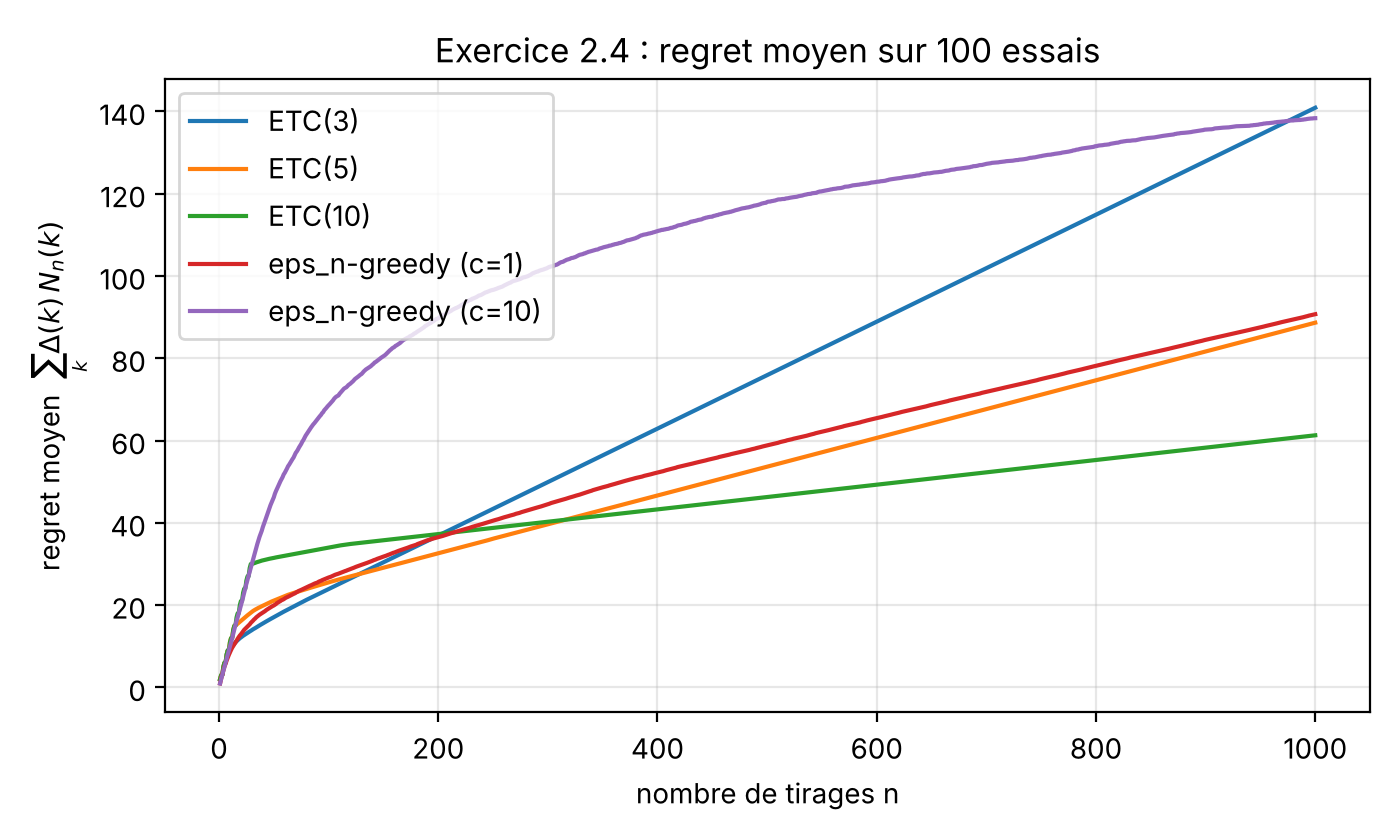
\includegraphics[width=0.72\textwidth]{ex24_regret.png}
  \caption{Regret moyen au cours du temps (100 essais).}
  \label{fig:regret}
\end{figure}

\subsection{La politique $\varepsilon_n$-greedy (question 3)}

Ici $\delta$ est le plus petit gap positif, donc $\delta = \min(2, 1) = 1$. Avec $c = 1$ et $K = 3$, on obtient $\varepsilon_n = \min(1, 3/n)$ : on explore a coup sûr pendant les 3 premiers tirages, puis avec probabilité $3/n$. Au total on explore en moyenne $\sum_n \varepsilon_n \approx 20$ fois sur 1000 tirages, donc environ 7 fois par machine, ce qui est très peu.

Sur 100 essais, 94 finissent sur la machine 3 et 6 sur la machine 2. Le regret moyen à $n = 1000$ vaut 90,7, presque comme ETC(5). On converge donc vers la bonne machine dans la grande majorité des essais, mais pas dans tous.

On peut presque retrouver ce chiffre à la main. La partie exploration du regret vaut $\frac1K \sum_k \Delta(k) \times \sum_n \varepsilon_n \approx 1 \times 20 = 20$. Le reste vient des 6\,\% d'essais restés sur la machine 2, qui coûtent chacun presque 1000, donc environ 60 en moyenne. On trouve $20 + 60 \approx 80$, pas très loin des 90,7 observés.

Par curiosité, nous avons aussi essayé $c = 10$, c'est-à-dire $\varepsilon_n = \min(1, 30/n)$. Là, 99 essais sur 100 finissent sur la machine 3, mais le regret est plus grand (138,3) parce qu'on explore beaucoup plus : $\sum_n \varepsilon_n \approx 135$, ce qui donne une partie exploration d'environ 135. Sur un horizon de 1000 seulement, explorer \og trop\fg{} coûte plus cher que se tromper de temps en temps. Sur un horizon beaucoup plus long ce serait sans doute l'inverse, car un essai bloqué sur la machine 2 fait grandir le regret de façon linéaire.

%======================================================================
\section{Exercice 3.1 : le robot vert}

\subsection{Le modèle}

Le robot est soit dans l'état \emph{high} (batterie chargée), soit dans l'état \emph{low}. Les données sont $r_w = 1$, $r_s = 5$, $r_b = -10$, $\gamma = 0,8$, $\alpha = 0,3$ et $\beta = 0,6$. En high, \emph{search} rapporte 5 et le robot reste en high avec probabilité 0,3 (sinon il passe en low), et \emph{wait} rapporte 1. En low, search rapporte aussi 5 et le robot reste en low avec probabilité 0,6, sinon il tombe en panne ($-10$) et repart en high, donc $\bar R_1(\text{low}, \text{search}) = 0,6 \times 5 - 0,4 \times 10 = -1$. Toujours en low, wait rapporte 1, et \emph{recharge} rapporte 0 et renvoie en high.

Un point nous a fait hésité : dans le poly, la récompense en cas de panne est $-r_b$. Avec $r_b = -10$ cela donnerait $+10$, et le robot aurait interêt à tomber en panne. Nous avons donc compris $r_b = -10$ comme \og la panne rapporte $-10$\fg{}. C'est le seul choix qui a du sens, mais nous préférons de le signaler.

\subsection{Itération de politique (question 1)}

On part de la politique w/w (attendre partout). À chaque étape, on évalue la politique en résolvant le système $2 \times 2$, puis on choisit dans chaque état l'action qui maximise $q$. En cas d'égalité on garde l'action actuelle, sinon l'algorithme pourrait tourner en rond.

\begin{table}[H]
  \centering
  \begin{tabular}{ccc}
    \toprule
    Étape & Politique (high / low) & $v_\Pi = (v(\text{high})\,;\, v(\text{low}))$ \\
    \midrule
    0 & w/w  & (5,00 ; 5,00) \\
    1 & s/w  & (10,26 ; 5,00) \\
    2 & s/re & (16,03 ; 12,82) \\
    \bottomrule
  \end{tabular}
  \caption{Les étapes de l'itération de politique.}
\end{table}

L'algorithme s'arrête après deux améliorations. La politique optimale est donc \textbf{s/re} : chercher quand la batterie est chargée, et recharger quand elle est faible, avec $v^* = (16,03\,;\,12,82)$. En low, les $q^*$ valent 12,82 pour recharger, 11,26 pour attendre et 10,28 pour chercher ; en high, 16,03 pour chercher et 13,82 pour attendre.

Intuitivement, chercher en low rapporte 5 dans 60\,\% des cas, mais la panne ($-10$) arrive dans 40\,\% des cas, ce qui donne $-1$ en moyenne tout de suite. Recharger ne rapporte rien sur le moment, mais ça renvoie en high, où l'on gagne 5 à chaque recherche.

\subsection{Estimation par Monte-Carlo (question 2a)}

À partir d'ici, on fait comme si on ne connaissait pas $\alpha$ et $\beta$, et on utilise seulement un simulateur qui tire l'état suivant au hasard. Le robot n'a pas d'état absorbant, donc il faut couper les trajectoires. Nous avons pris $T = 60$ pas : le reste de la somme est au plus $10 \times 0,8^{60} / (1 - 0,8) \approx 10^{-4}$, ce qui est négligable. Pour chaque politique et chaque état de départ, on fait la moyenne de 2000 retours $G^T(s) = \sum_{k<T} \gamma^k R_{k+1}$.

\begin{table}[H]
  \centering
  \begin{tabular}{cccc}
    \toprule
    Politique & $v$ exacte (high ; low) & Monte-Carlo, départ high & Monte-Carlo, départ low \\
    \midrule
    s/w  & 10,26 ; 5,00  & $10,24 \pm 0,09$ & $5,00 \pm 0,00$ \\
    s/s  & 9,44 ; 3,89   & $9,49 \pm 0,27$  & $4,08 \pm 0,34$ \\
    s/re & 16,03 ; 12,82 & $16,06 \pm 0,07$ & $12,85 \pm 0,06$ \\
    \bottomrule
  \end{tabular}
  \caption{Monte-Carlo avec 2000 trajectoires ($\pm$ = demi-largeur de l'intervalle de confiance à 95\,\%).}
  \label{tab:mc}
\end{table}

Toutes les vraies valeurs sont dans l'interval de confiance à 95\,\%. La politique s/s est la plus difficile à estimer ($\pm 0,3$), parce que les pannes à $-10$ rendent les retours très variables. Pour s/w en partant de low, il n'y a aucun hasard (le robot attend pour toujours et gagne 1 à chaque pas), donc on trouve exactement 5. En traçant la moyenne en fonction du nombre de trajectoires, on voit que quelques centaines de trajectoires suffit déjà.

\subsection{TD(0) (question 2b)}

La mise à jour est $V(S) \leftarrow V(S) + \eta\,\big(R + \gamma V(S') - V(S)\big)$. Au début nous avions lancé une seule longue trajectoire, mais pour s/w ça ne marche pas : une fois en low, le robot attend pour toujours et $V(\text{high})$ n'est plus jamais mis à jour. Nous avons donc fait 2000 épisodes de 50 pas, chacun partant d'un état tiré au hasard, soit 100\,000 mises à jour en tout. Nous avons testé $\eta = 0,5$, $0,1$ et $0,01$, et aussi un pas décroissant $\eta_n = 1/(\text{nombre de visites de l'état})$.

\begin{table}[H]
  \centering
  \begin{tabular}{cccc}
    \toprule
    Pas $\eta$ & s/w & s/s & s/re \\
    \midrule
    0,5  & 0,80 & 7,77 & 1,08 \\
    0,1  & 0,42 & 2,14 & 0,34 \\
    0,01 & 0,11 & 0,46 & 0,12 \\
    $1/n$ & 0,47 & 0,39 & 1,28 \\
    \bottomrule
  \end{tabular}
  \caption{Erreur $\max_s |V(s) - v_\Pi(s)|$, moyennée sur les 500 derniers épisodes.}
\end{table}

Sur la figure~\ref{fig:td31} (pour s/re), on voit qu'avec un pas constant l'erreur descend vite, puis reste sur un \og plateau\fg{} de bruit. Plus $\eta$ est grand, plus le plateau est haut : environ 1 pour $\eta = 0,5$, 0,3 pour $\eta = 0,1$ et 0,1 pour $\eta = 0,01$. En contrepartie, $\eta = 0,01$ met une centaine d'épisodes à démarrer.

Le pas $1/n$ vérifie $\sum \eta_n = \infty$ et $\sum \eta_n^2 < \infty$, donc en théorie il converge. Mais en pratique il est trop lent ici : après 100\,000 mises à jour, l'erreur pour s/re vaut encore 1,3. Le pas devient petit trop tôt, alors que les premières estimations (parti de 0) sont encore mauvaises.

Comme pour Monte-Carlo, s/s est de nouveau la politique la plus difficile, et avec $\eta = 0,5$ l'erreur moyenne vaut 7,8. Avec $\eta = 0,01$ par contre, TD(0) donne $V = (10,22\,;\,5,00)$ pour s/w, $(9,37\,;\,4,00)$ pour s/s et $(16,10\,;\,12,88)$ pour s/re, ce qui est proche des valeurs exactes du tableau~\ref{tab:mc}.

\begin{figure}[H]
  \centering
  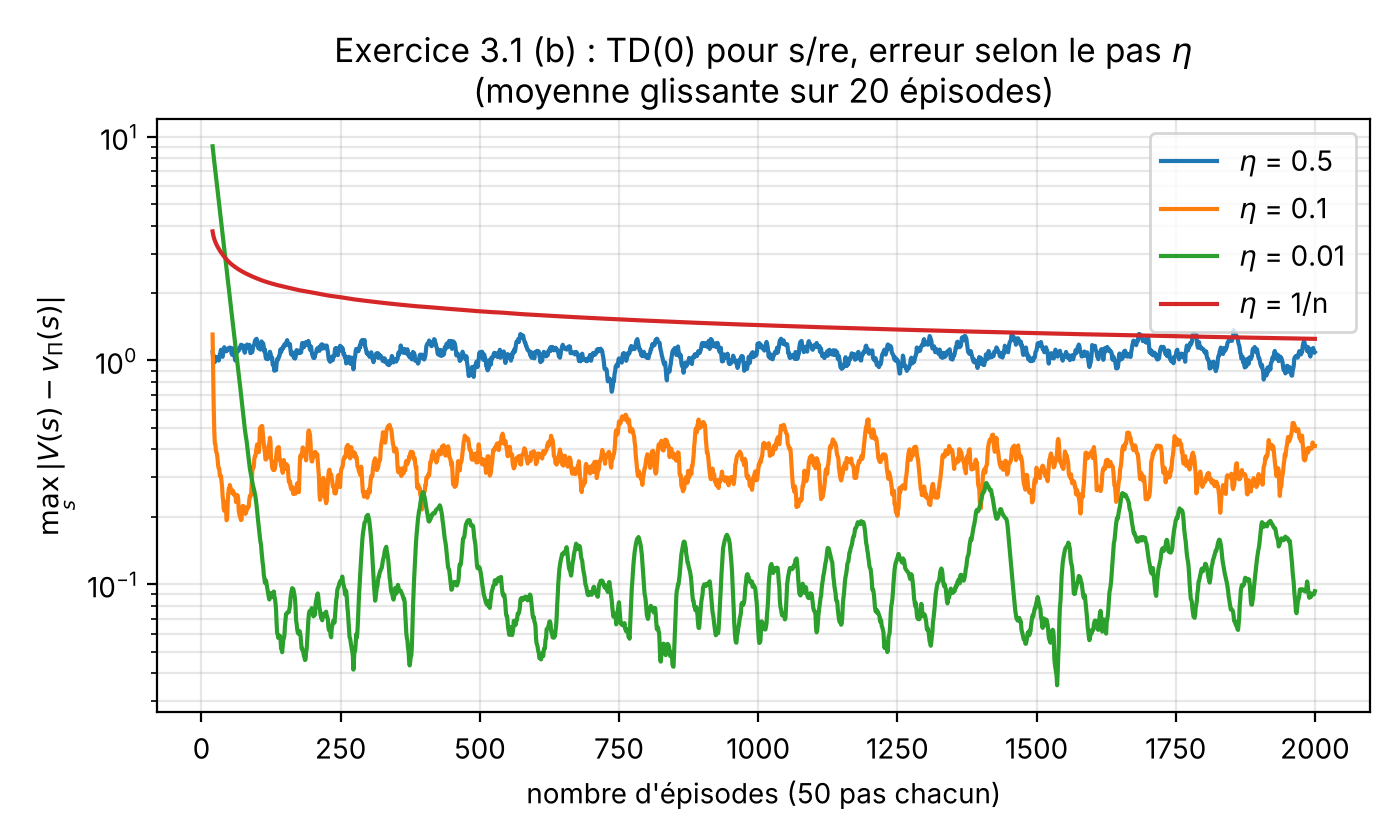
\includegraphics[width=0.72\textwidth]{ex31_td0.png}
  \caption{Erreur de TD(0) pour s/re selon le pas (échelle logarithmique).}
  \label{fig:td31}
\end{figure}

\subsection{Contrôle par Monte-Carlo $\varepsilon$-greedy (question 2c)}

Nous avons suivi l'algorithme 4 du chapitre 3 avec $\varepsilon = 0,1$. On génère une trajectoire avec la politique $\varepsilon$-greedy actuelle, on met à jour $Q(s, a)$ par la moyenne des retours observés après chaque couple $(s, a)$, puis on rend la politique gloutonne (avec $\varepsilon$) dans les états visités. Nous avons fait 3000 trajectoires de 100 pas avec un départ au hasard, et on garde seulement les visites des 60 premiers pas, pour que chaque retour soit calculé sur au moins 40 pas.

Il y a eu un petit problème au début. Dans le poly, $G$ est \og la récompense immédiatement obtenue en quittant $(s, a)$\fg{}. Nous avons d'abord codé exactement ça, et on a obtenu la politique s/w : en low, attendre ($+1$) bat recharger (0) et chercher ($-1$) si on regarde seulement le pas suivant. C'est une politique myope, pas l'optimale. Avec le vrai retour $G_t = \sum_k \gamma^k R_{t+k+1}$, on retrouve bien s/re.

\begin{table}[H]
  \centering
  \begin{tabular}{ccc}
    \toprule
    $(s, a)$ & $Q$ estimé (MC $\varepsilon$-greedy) & $q^*$ (avec le modèle) \\
    \midrule
    high, search  & 15,53 & 16,03 \\
    high, wait    & 12,76 & 13,82 \\
    low, search   & 9,49  & 10,28 \\
    low, wait     & 10,47 & 11,26 \\
    low, recharge & 12,34 & 12,82 \\
    \bottomrule
  \end{tabular}
  \caption{Valeurs état/action après 3000 trajectoires. La politique gloutonne obtenue est s/re.}
\end{table}

Les valeurs estimées sont un peu en dessous de $q^*$. C'est normal, car ce sont les valeurs de la politique $\varepsilon$-greedy, qui choisit encore une moins bonne action de temps en temps (environ 7\,\% du temps en low). Mais l'ordre des actions est le bon dans les deux états, et c'est ça qui compte pour la politique. La figure~\ref{fig:mcctrl} montre que recharger passe devant dès les premières dizaines de trajectoires.

\begin{figure}[H]
  \centering
  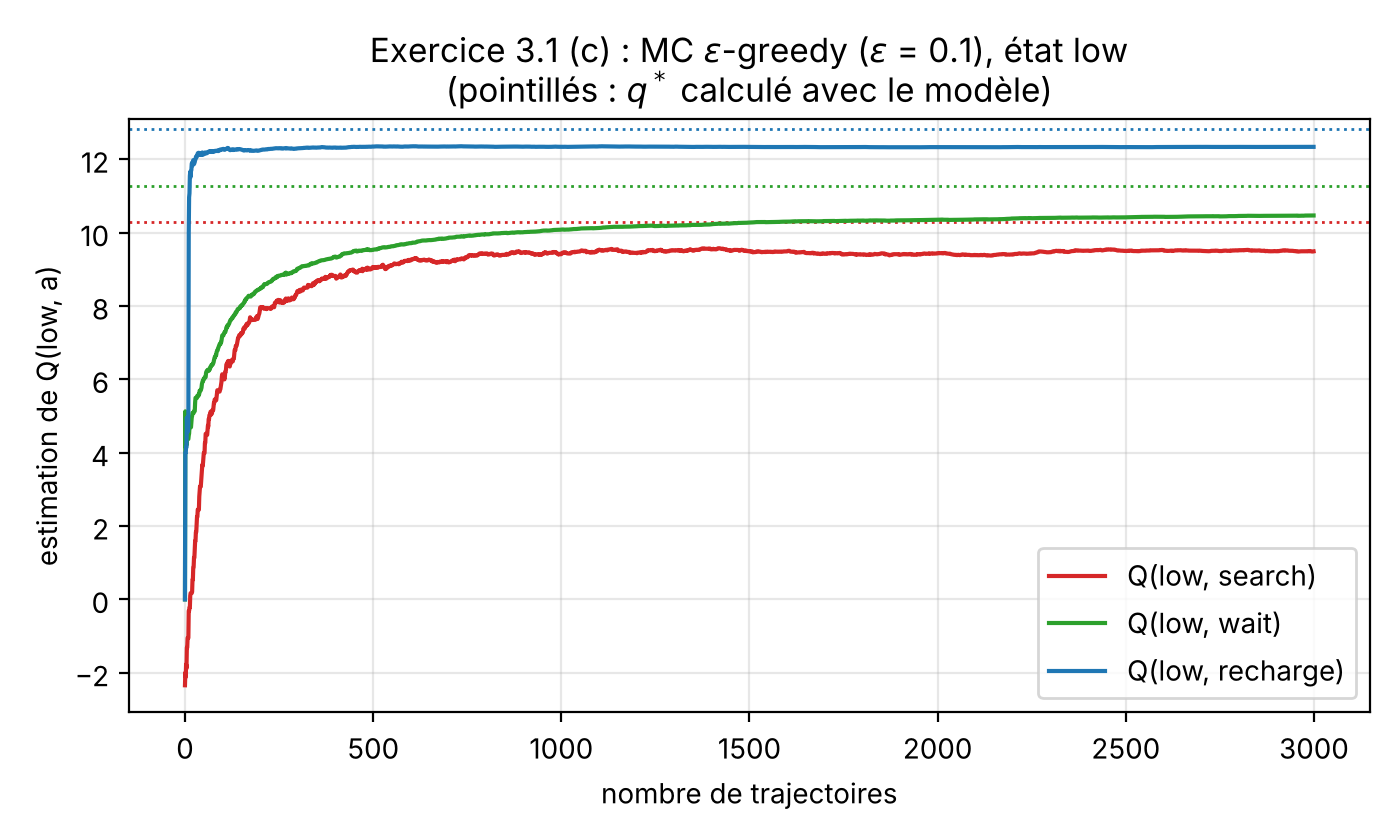
\includegraphics[width=0.68\textwidth]{ex31_mc_controle.png}
  \caption{Évolution des estimations de $Q(\text{low}, a)$ pendant l'algorithme.}
  \label{fig:mcctrl}
\end{figure}

%======================================================================
\section{Exercice 3.2 : le dilemme de l'étudiant}

\subsection{Le modèle et les valeurs exactes}

Il y a sept états, et 5, 6 et 7 sont absorbants. Les deux actions sont R (se reposer) et W (travailler). Nous avons lu les probabilités et les récompenses sur la figure du cours (tableau~\ref{tab:modele}). Comme dans le cours, la récompense $r(s')$ est reçue en arrivant dans $s'$, et tout vaut 0 après un état absorbant, donc $v(5) = v(6) = v(7) = 0$. On prend $\gamma = 0,8$.

\begin{table}[H]
  \centering
  \begin{tabular}{ccccc}
    \toprule
    État ($r$) & R : état suivant (prob.) & $\bar R_1(s, \text{R})$ & W : état suivant (prob.) & $\bar R_1(s, \text{W})$ \\
    \midrule
    1 ($r = 0$)   & 1 (0,5) ; 2 (0,5) & 0,5  & 1 (0,5) ; 3 (0,5) & $-0,5$ \\
    2 ($r = 1$)   & 2 (0,6) ; 5 (0,4) & $-3,4$ & 1 (0,3) ; 3 (0,7) & $-0,7$ \\
    3 ($r = -1$)  & 2 (0,4) ; 3 (0,6) & $-0,2$ & 3 (0,5) ; 4 (0,5) & $-5,5$ \\
    4 ($r = -10$) & 6 (0,9) ; 4 (0,1) & 89   & 7 (1)             & $-1000$ \\
    \bottomrule
  \end{tabular}
  \caption{Le modèle lu sur la figure ($r(5) = -10$, $r(6) = 100$, $r(7) = -1000$).}
  \label{tab:modele}
\end{table}

Pour avoir une référence, nous avons calculé avec le modèle la valeur exacte de SWWS (R en 1, W en 2 et 3, R en 4) et la politique optimale, par itération de politique.

\begin{table}[H]
  \centering
  \begin{tabular}{ccccc}
    \toprule
    État & $v_{\text{SWWS}}$ & $v^*$ & $q^*(s, \text{R})$ & $q^*(s, \text{W})$ \\
    \midrule
    1 & 25,03 & 36,05 & 30,49 & 36,05 \\
    2 & 36,29 & 38,93 & 15,29 & 38,93 \\
    3 & 55,33 & 55,33 & 38,82 & 55,33 \\
    4 & 96,74 & 96,74 & 96,74 & $-1000,00$ \\
    \bottomrule
  \end{tabular}
  \caption{Valeurs exactes (calculées avec le modèle).}
\end{table}

La politique optimale est \textbf{W/W/W/R} : travailler dans les états 1, 2 et 3, et se reposer en 4. SWWS ne diffère que dans l'état 1, où elle se repose, et on le paie : $v_{\text{SWWS}}(1) = 25,0$ contre $v^*(1) = 36,1$. Se reposer en 1 rapporte un peu tout de suite ($+0,5$ contre $-0,5$), mais ça retarde l'arrivée en 4 puis en 6, où se trouve la récompense de 100.

\subsection{TD(0) pour la politique SWWS (question 1)}

Chaque épisode part d'un état tiré au hasard parmi 1, 2, 3 et 4, et s'arrête quand on arrive dans un état absorbant. Nous avons fait 5000 épisodes pour $\alpha = 0,5$, $0,1$, $0,01$ et pour le pas décroissant $1/n$.

\begin{table}[H]
  \centering
  \begin{tabular}{cccccc}
    \toprule
    $\alpha$ & $V(1)$ & $V(2)$ & $V(3)$ & $V(4)$ & Erreur moyenne \\
    \midrule
    valeur exacte & 25,03 & 36,29 & 55,33 & 96,74 & --- \\
    0,5  & 29,90 & 39,21 & 60,91 & 96,14 & 10,94 \\
    0,1  & 27,20 & 37,14 & 56,08 & 99,17 & 4,27 \\
    0,01 & 25,47 & 37,74 & 56,40 & 97,91 & 1,28 \\
    $1/n$ & 20,29 & 33,40 & 54,13 & 96,75 & 4,83 \\
    \bottomrule
  \end{tabular}
  \caption{TD(0) après 5000 épisodes (erreur $\max_s |V(s) - v_{\text{SWWS}}(s)|$, moyennée sur les 500 derniers épisodes).}
\end{table}

Comme pour le robot, $\alpha = 0,01$ est le meilleur compromis (erreur moyenne 1,3). Les erreurs sont plus grands que pour le robot, parce que les récompenses le sont aussi (100 en 6, $-10$ en 4) : avec $\alpha = 0,5$, l'estimation saute de $\pm 10$ d'un épisode à l'autre. Le pas $1/n$ est encore trop lent, surtout pour les états 1 et 2, qui sont loin des récompenses et dépendent des estimations des autres états.

\begin{figure}[H]
  \centering
  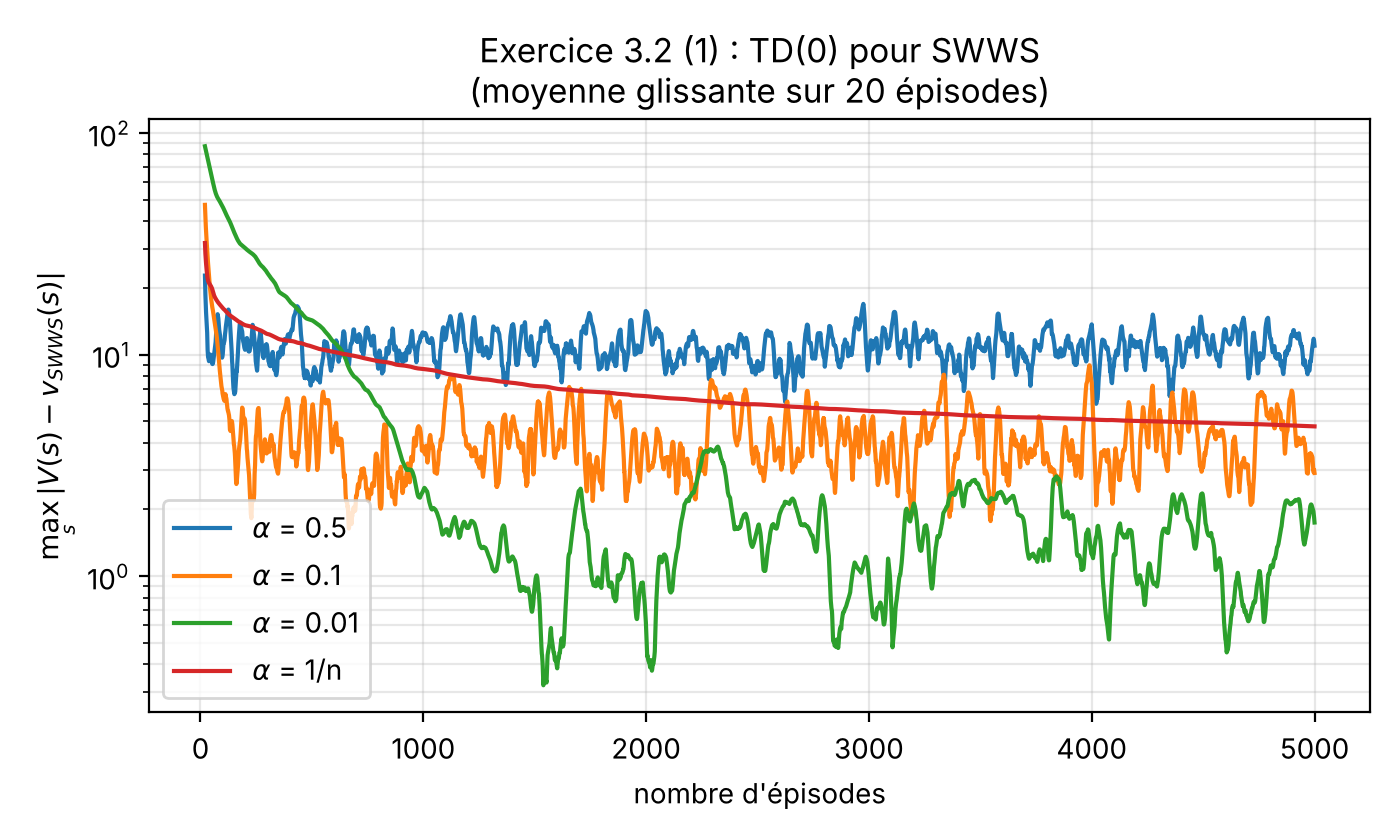
\includegraphics[width=0.7\textwidth]{ex32_td0.png}
  \caption{Erreur de TD(0) pour SWWS selon $\alpha$ (échelle logarithmique).}
\end{figure}

\subsection{Q-learning (question 2)}

Nous avons codé l'algorithme 6 du chapitre 3 : on choisit l'action par $\varepsilon$-greedy ($\varepsilon = 0,1$), mais on met à jour avec la cible $R + \gamma \max_a Q(S', a)$. Nous avons fait 20\,000 épisodes avec un départ au hasard dans $\{1, 2, 3, 4\}$, pour $\alpha = 0,5$, $0,1$ et $0,01$.

À la fin, les trois valeurs de $\alpha$ donnent la politique W/W/W/R, c'est-à-dire la politique optimale, mais le chemin n'est pas du tout le même (figure~\ref{fig:ql}). Avec $\alpha = 0,5$, la politique gloutonne change souvent : les $Q$ sont trop bruités, et dans l'état 1 l'écart entre $Q(1, \text{R})$ et $Q(1, \text{W})$ (environ 5,6 en théorie) est parfois inversé. Avec $\alpha = 0,1$, c'est presque toujours la bonne politique, avec juste quelques changements de temps en temps.

Avec $\alpha = 0,01$ c'est différent : la politique est fausse pendant environ 3539 épisodes, puis elle ne bouge plus. Au début, l'information \og il y a 100 en 6\fg{} remonte très lentement vers l'état 1, et l'étudiant préfère se reposer (récompense immédiate $+0,5$). Une fois que la valeur est remonté, la politique devient stable.

\begin{figure}[H]
  \centering
  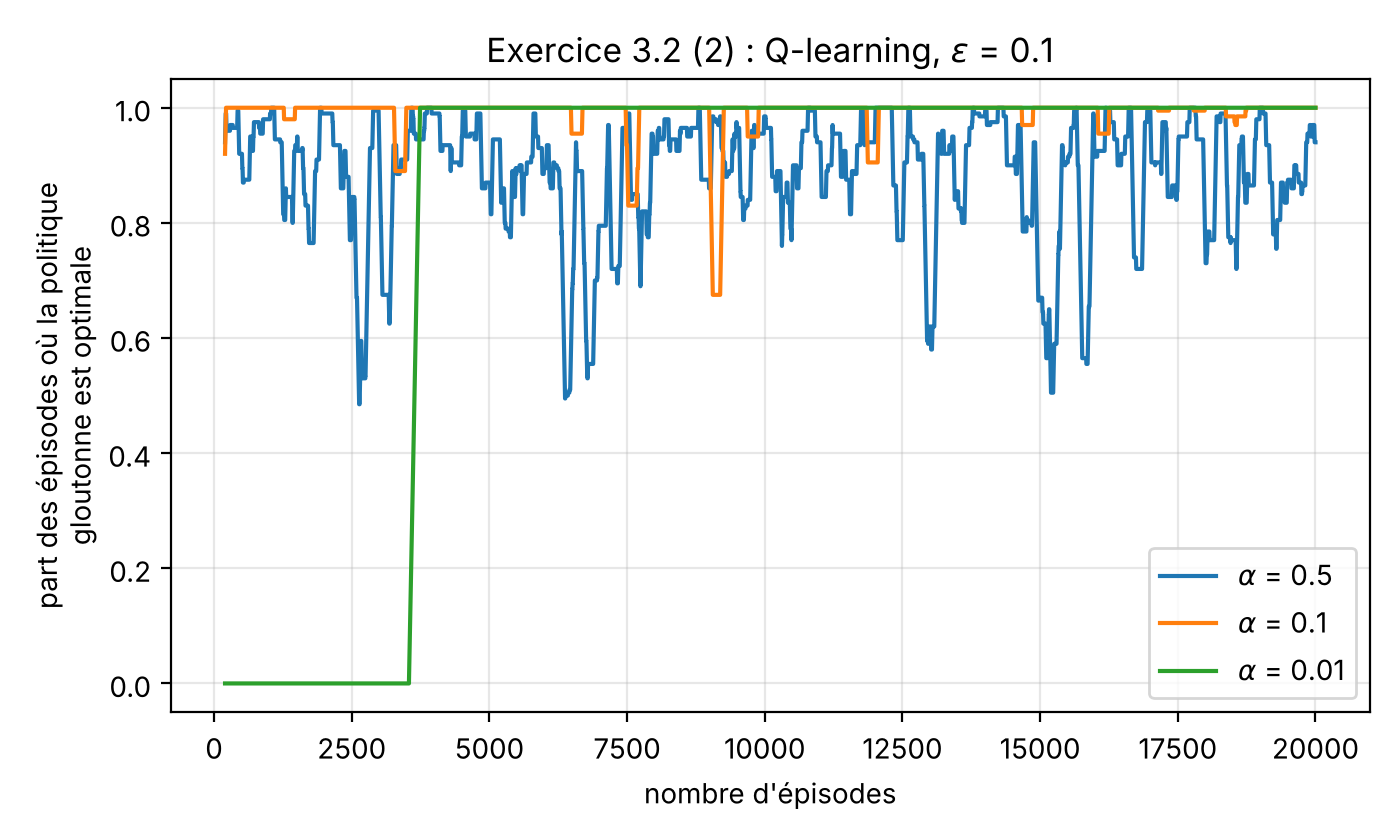
\includegraphics[width=0.7\textwidth]{ex32_qlearning.png}
  \caption{Part des épisodes où la politique gloutonne est la politique optimale (moyenne glissante sur 200 épisodes).}
  \label{fig:ql}
\end{figure}

\begin{table}[H]
  \centering
  \begin{tabular}{cccc}
    \toprule
    $(s, a)$ & $Q$, $\alpha = 0,01$ & $Q$, $\alpha = 0,1$ & $q^*$ \\
    \midrule
    1, R & 30,36 & 31,75 & 30,49 \\
    1, W & 37,34 & 40,33 & 36,05 \\
    2, R & 10,32 & 19,93 & 15,29 \\
    2, W & 38,95 & 40,72 & 38,93 \\
    3, R & 38,62 & 41,83 & 38,82 \\
    3, W & 55,69 & 57,17 & 55,33 \\
    4, R & 96,51 & 99,21 & 96,74 \\
    4, W & $-999,99$ & $-1000,00$ & $-1000,00$ \\
    \bottomrule
  \end{tabular}
  \caption{$Q$ après 20\,000 épisodes de Q-learning, comparé à $q^*$.}
\end{table}

Avec $\alpha = 0,01$, les $Q$ sont très proches de $q^*$, sauf $Q(2, \text{R})$ (10,3 au lieu de 15,3). Cette action n'est presque jamais choisi, puisque $\varepsilon$-greedy prend W en 2 dans 95\,\% des cas, donc elle est rarement mise à jour. Ça ne gêne pas pour trouver la politique, car elle reste nettement moins bonne que W.

%======================================================================
\section*{Conclusion}

Ce projet nous a permis de voir concrètement des choses que nous avions vu en cours de façon plus théorique.

Pour les bandits, le compromis exploration / exploitation se voit très bien sur les chiffres. Avec trop peu d'exploration (ETC(3), ou $\varepsilon_n$-greedy avec $c = 1$), on reste parfois bloqué sur une mauvaise machine, et avec beaucoup d'exploration ($c = 10$) c'est l'exploration elle-même qui coûte cher.

Pour l'évaluation d'une politique, Monte-Carlo et TD(0) retrouvent les valeurs exactes, mais pour TD(0) le choix du pas est très important, et le pas $1/n$ de la théorie est trop lent dans nos exemples. Enfin, les méthodes sans modèle (MC $\varepsilon$-greedy et Q-learning) retrouvent les mêmes politiques optimales que l'itération de politique, c'est-à-dire s/re pour le robot et W/W/W/R pour l'étudiant.

Une limite de notre travail est que, pour les exercices 3.1 et 3.2, nous n'avons utilisé qu'une graine par expérience. Il faudrait répeter ces expériences plusieurs fois, comme pour l'exercice 2.4, pour avoir des barres d'erreur.

%======================================================================
\clearpage
\appendix
\section{Code des algorithmes}

Pour ne pas alourdir le rapport, nous mettons ici seulement les fonctions qui codent les algorithmes. Le code complet (statistiques, figures, calcul des valeurs exactes) est dans l'archive jointe au rapport (\texttt{rl-projet-m2.zip}). Les numéros de ligne sont ceux des fichiers complets, et chaque fichier se lance avec \texttt{python nom\_du\_fichier.py}.

\subsection{\texttt{ex24\_bandits.py} : ETC($m$) et $\varepsilon_n$-greedy}

\begin{lstlisting}[firstnumber=35]
def argmax_aleatoire(valeurs, rng):
    """argmax, mais en cas d'égalité on tire au sort parmi les meilleurs
    (c'est le « une des machines » du poly)."""
    meilleurs = np.flatnonzero(valeurs == valeurs.max())
    return rng.choice(meilleurs)
\end{lstlisting}

\begin{lstlisting}[firstnumber=42]
# ETC(m), def 4.5 du chap 2
def etc(m, rng, n=N_TIRAGES, recompenses_forcees=None):
    """Joue ETC(m) pendant n tirages.

    Exploration : on joue 1, 2, 3, 1, 2, 3, ... (m fois chaque machine).
    Ensuite : A_i dans argmax mu_hat_{i-1}. Attention dans le poly les
    moyennes continuent d'être mise à jour après l'exploration (c'est
    une politique « greedy » à partir de mK + 1).

    recompenses_forcees : liste optionnelle qui remplace les premières
    récompenses (ça sert juste a tester l'evenement de la question 2a).
    """
    somme = np.zeros(K)  # somme des récompenses de chaque machine
    nb = np.zeros(K)  # N_n(k) : nombre de fois où on a joué k
    actions = np.empty(n, dtype=int)
    recompenses = np.empty(n)

    for i in range(n):
        if i < m * K:
            a = i % K  # exploration : 1, 2, 3, 1, 2, 3...
        else:
            mu_hat = somme / nb  # ici nb > 0 partout, pas de division par 0
            a = argmax_aleatoire(mu_hat, rng)

        if recompenses_forcees is not None and i < len(recompenses_forcees):
            x = recompenses_forcees[i]
        else:
            x = rng.poisson(LAMBDAS[a])

        # on met a jour seulement la machine qu'on a joué
        somme[a] += x
        nb[a] += 1
        actions[i] = a
        recompenses[i] = x
    return actions, recompenses
\end{lstlisting}

\begin{lstlisting}[firstnumber=79]
# eps_n-greedy (def 4.9 chap 2)
def eps_n_greedy(c, rng, n=N_TIRAGES, delta=1.0):
    """eps_n = min(1, cK / (delta^2 n)).

    Avec probabilité eps_n on explore (machine uniforme), sinon on joue
    une machine de argmax mu_hat. Une machine jamais jouée a mu_hat = 0
    (c'est une convention a nous, de toute façon on explore au tout debut).
    """
    somme = np.zeros(K)
    nb = np.zeros(K)
    actions = np.empty(n, dtype=int)
    recompenses = np.empty(n)

    for i in range(n):
        t = i + 1  # t commence a 1 sinon eps = c*K/0
        eps = min(1.0, c * K / (delta ** 2 * t))
        if rng.random() < eps:
            a = rng.integers(K)  # on explore
        else:
            mu_hat = np.divide(somme, nb, out=np.zeros(K), where=nb > 0)
            a = argmax_aleatoire(mu_hat, rng)  # on exploite
        x = rng.poisson(LAMBDAS[a])
        somme[a] += x
        nb[a] += 1
        actions[i] = a
        recompenses[i] = x
    return actions, recompenses
\end{lstlisting}

\subsection{\texttt{ex31\_robot.py} : itération de politique, simulateur, MC, TD(0), MC $\varepsilon$-greedy}

\begin{lstlisting}[firstnumber=79]
# Q1 : iteration de politique
def iteration_politique(depart):
    politique = dict(depart)
    historique = []
    while True:
        v = valeur_exacte(politique)  # évaluation
        q = q_depuis_v(v)
        nouvelle = {}
        for s in (HIGH, LOW):  # amélioration gloutonne
            meilleure = max(ACTIONS[s], key=lambda a: q[(s, a)])
            # si egalité on garde l'action actuelle, sinon ça peut boucler a l'infini
            if np.isclose(q[(s, meilleure)], q[(s, politique[s])]):
                meilleure = politique[s]
            nouvelle[s] = meilleure
        historique.append({"politique": f"{politique[HIGH]}/{politique[LOW]}",
                           "v": [round(float(x), 4) for x in v]})
        if nouvelle == politique:  # plus rien ne change donc on s'arrete
            return politique, v, historique
        politique = nouvelle
\end{lstlisting}

\begin{lstlisting}[firstnumber=100]
# simulateur : c'est la seule chose qu'on a le droit d'utiliser en Q2
def un_pas(s, a, rng):
    """Tire l'état suivant et la récompense (comme si on regardait le robot)."""
    u = rng.random()
    cumul = 0.0
    for p, s2, r in TRANSITIONS[(s, a)]:
        cumul += p
        if u < cumul:
            return s2, r
    return s2, r  # au cas ou cumul = 0.9999... a cause des arrondis
\end{lstlisting}

\begin{lstlisting}[firstnumber=116]
def retour_mc(politique, s, rng, T=T_HORIZON):
    """G^T(s) = sum_{k<T} gamma^k R_{k+1} en partant de s."""
    G, remise = 0.0, 1.0
    for _ in range(T):
        s, r = un_pas(s, politique[s], rng)
        G += remise * r
        remise *= GAMMA
    return G
\end{lstlisting}

\begin{lstlisting}[firstnumber=138]
# Q2b : TD(0)
def td0(politique, eta, n_episodes, rng, T=50, v_exacte=None):
    """TD(0) : V(S) <- V(S) + eta (R + gamma V(S') - V(S)).

    Le robot n'a pas d'état absorbant, donc on coupe en épisodes de T pas,
    chacun partant d'un état tiré au hasard. C'est necessaire pour s/w :
    en low le robot attend pour toujours, sinon on reverrait jamais high.
    eta peut être un nombre, ou "1/n" (pas 1 / nombre de visites de l'état).
    """
    V = np.zeros(2)
    visites = np.zeros(2)
    erreurs = []
    for _ in range(n_episodes):
        s = rng.integers(2)
        for _ in range(T):
            s2, r = un_pas(s, politique[s], rng)
            visites[s] += 1
            pas = 1.0 / visites[s] if eta == "1/n" else eta
            V[s] += pas * (r + GAMMA * V[s2] - V[s])
            s = s2
        if v_exacte is not None:
            erreurs.append(np.max(np.abs(V - v_exacte)))
    return V, np.array(erreurs)
\end{lstlisting}

\begin{lstlisting}[firstnumber=163]
# Q2c : online MC eps-greedy (algo 4 du chap 3)
def mc_eps_greedy(eps, n_traj, rng, T=100, t_max_visite=60, recompense_immediate=False):
    """Contrôle par Monte-Carlo avec une politique eps-greedy.

    Dans le poly, G = « récompense immédiatement obtenue en quittant (s, a) ».
    On a essayé ça (recompense_immediate=True) mais on trouve s/w : la
    politique ne regarde pas l'avenir. Par défaut on prend donc le vrai
    retour G_t = sum_k gamma^k R_{t+k+1}, calculé sur la fin de la trajectoire.
    On ne garde que les visites t < t_max_visite pour que le retour soit
    calculé sur au moins 40 pas (0.8^40 ~ 1e-4).
    """
    Q = {(s, a): 0.0 for s in (HIGH, LOW) for a in ACTIONS[s]}
    # au lieu de garder toute la liste Returns(s, a) on met juste la moyenne a jour
    # (ça donne la meme chose et c'est beaucoup plus rapide)
    nb_retours = {cle: 0 for cle in Q}
    gloutonne = {HIGH: "search", LOW: "search"}  # politique de depart
    suivi = []  # pour la figure

    def choisir(s):
        # pi(a|s) = 1 - eps + eps/|A(s)| pour l'action gloutonne, eps/|A(s)| sinon
        if rng.random() < eps:
            return ACTIONS[s][rng.integers(len(ACTIONS[s]))]
        return gloutonne[s]

    for _ in range(n_traj):
        # 1) on genere une trajectoire avec la politique actuel
        s = rng.integers(2)
        traj = []
        for _ in range(T):
            a = choisir(s)
            s2, r = un_pas(s, a, rng)
            traj.append((s, a, r))
            s = s2
        # 2) on calcul les retours en partant de la fin
        G = 0.0
        G_t = [0.0] * T
        for t in range(T - 1, -1, -1):
            G = traj[t][2] + GAMMA * G
            G_t[t] = G
        # 3) MAJ de Q = moyenne des retours (toutes les visites)
        for t in range(t_max_visite):
            s_t, a_t, r_t = traj[t]
            cible = r_t if recompense_immediate else G_t[t]
            nb_retours[(s_t, a_t)] += 1
            # moyenne incrementale : nouvelle = ancienne + (cible - ancienne) / n
            Q[(s_t, a_t)] += (cible - Q[(s_t, a_t)]) / nb_retours[(s_t, a_t)]
        # 4) amelioration : on prend l'action gloutonne dans les etats visités
        for s_vu in {x[0] for x in traj[:t_max_visite]}:
            gloutonne[s_vu] = max(ACTIONS[s_vu], key=lambda a: Q[(s_vu, a)])
        suivi.append({cle: Q[cle] for cle in Q})
    return Q, gloutonne, suivi
\end{lstlisting}

\subsection{\texttt{ex32\_etudiant.py} : TD(0) et Q-learning}

\begin{lstlisting}[firstnumber=107]
# Q1 : TD(0) pour SWWS
def td0(politique, alpha, n_episodes, rng, v_exacte):
    """Chaque épisode part d'un état tiré au hasard dans {1, 2, 3, 4}
    et s'arrête quand on tombe dans un état absorbant."""
    V = {s: 0.0 for s in ETATS}  # V reste a 0 sur 5, 6, 7
    visites = {s: 0 for s in NON_ABS}
    erreurs = []
    for _ in range(n_episodes):
        s = int(rng.choice(NON_ABS))
        for _ in range(T_MAX):
            if s in ABSORBANTS:
                break
            s2, rec = un_pas(s, politique[s], rng)
            visites[s] += 1
            pas = 1.0 / visites[s] if alpha == "1/n" else alpha
            V[s] += pas * (rec + GAMMA * V[s2] - V[s])
            s = s2
        erreurs.append(max(abs(V[s] - v_exacte[s]) for s in NON_ABS))
    return V, np.array(erreurs)
\end{lstlisting}

\begin{lstlisting}[firstnumber=128]
# Q2 : Q-learning (algo 6 du chap 3)
def q_learning(alpha, eps, n_episodes, rng, politique_opt):
    """On explore avec eps-greedy, mais on met à jour avec max_a Q(S', a)."""
    Q = {(s, a): 0.0 for s in ETATS for a in ACTIONS}  # Q = 0 sur les etats absorbants
    bonne_politique = []  # 1 si la politique gloutonne est deja la bonne
    for _ in range(n_episodes):
        s = int(rng.choice(NON_ABS))
        for _ in range(T_MAX):
            if s in ABSORBANTS:
                break
            # eps-greedy (si egalité on tire au hasard)
            if rng.random() < eps:
                a = ACTIONS[rng.integers(2)]
            else:
                qs = [Q[(s, b)] for b in ACTIONS]
                a = ACTIONS[rng.integers(2)] if qs[0] == qs[1] else ACTIONS[int(np.argmax(qs))]
            s2, rec = un_pas(s, a, rng)
            cible = rec + GAMMA * max(Q[(s2, b)] for b in ACTIONS)
            Q[(s, a)] += alpha * (cible - Q[(s, a)])
            s = s2
        gloutonne = {x: max(ACTIONS, key=lambda b: Q[(x, b)]) for x in NON_ABS}
        bonne_politique.append(gloutonne == politique_opt)
    return Q, gloutonne, np.array(bonne_politique)
\end{lstlisting}

\end{document}
